
% this file is called up by thesis.tex
% content in this file will be fed into the main document

%: ----------------------- introduction file header -----------------------
\chapter{Introduction}

% the code below specifies where the figures are stored
\ifpdf
    \graphicspath{{1_introduction/figures/PNG/}{1_introduction/figures/PDF/}{1_introduction/figures/}}
\else
    \graphicspath{{1_introduction/figures/EPS/}{1_introduction/figures/}}
\fi

% ----------------------------------------------------------------------
%: ----------------------- introduction content ----------------------- 
% ----------------------------------------------------------------------



%: ----------------------- HELP: latex document organisation
% the commands below help you to subdivide and organise your thesis
%    \chapter{}       = level 1, top level
%    \section{}       = level 2
%    \subsection{}    = level 3
%    \subsubsection{} = level 4
% note that everything after the percentage sign is hidden from output



\section{Context} 

% We have a separate previous work section we will ignore most of the different
% related literature in the introduction.

% Problem

The amount of data being generated and processed worldwide is growing rapidly.
Meanwhile the prevalent Von Nuemann computer architecture requires all data to
be moved to system memory before it can be processed
\cite{2018-neumann-bottleneck}. Until recently storage devices such as hard-disk
drives (HDDs) or solid-state drives (SSDs) have only been passively storing
data. With the increasing bandwidth persistent storage devices like SSDs achieve
this excessive data movement to memory is increasingly becoming a bottleneck
\cite{2014-micro-ndp}. Similarly, the CPU generational performance
improvements \cite{2016-western-digital} as well as link speeds of interconnects
are stagnating compared to NAND flash bandwidth \cite{10.1145/3286588}, the
underlying technology enabling modern SSDs. The typical proportions of this
large bandwidth gap are demonstrated in figure \ref{figure:storagebottleneck}.

\begin{figure}
    \centering
	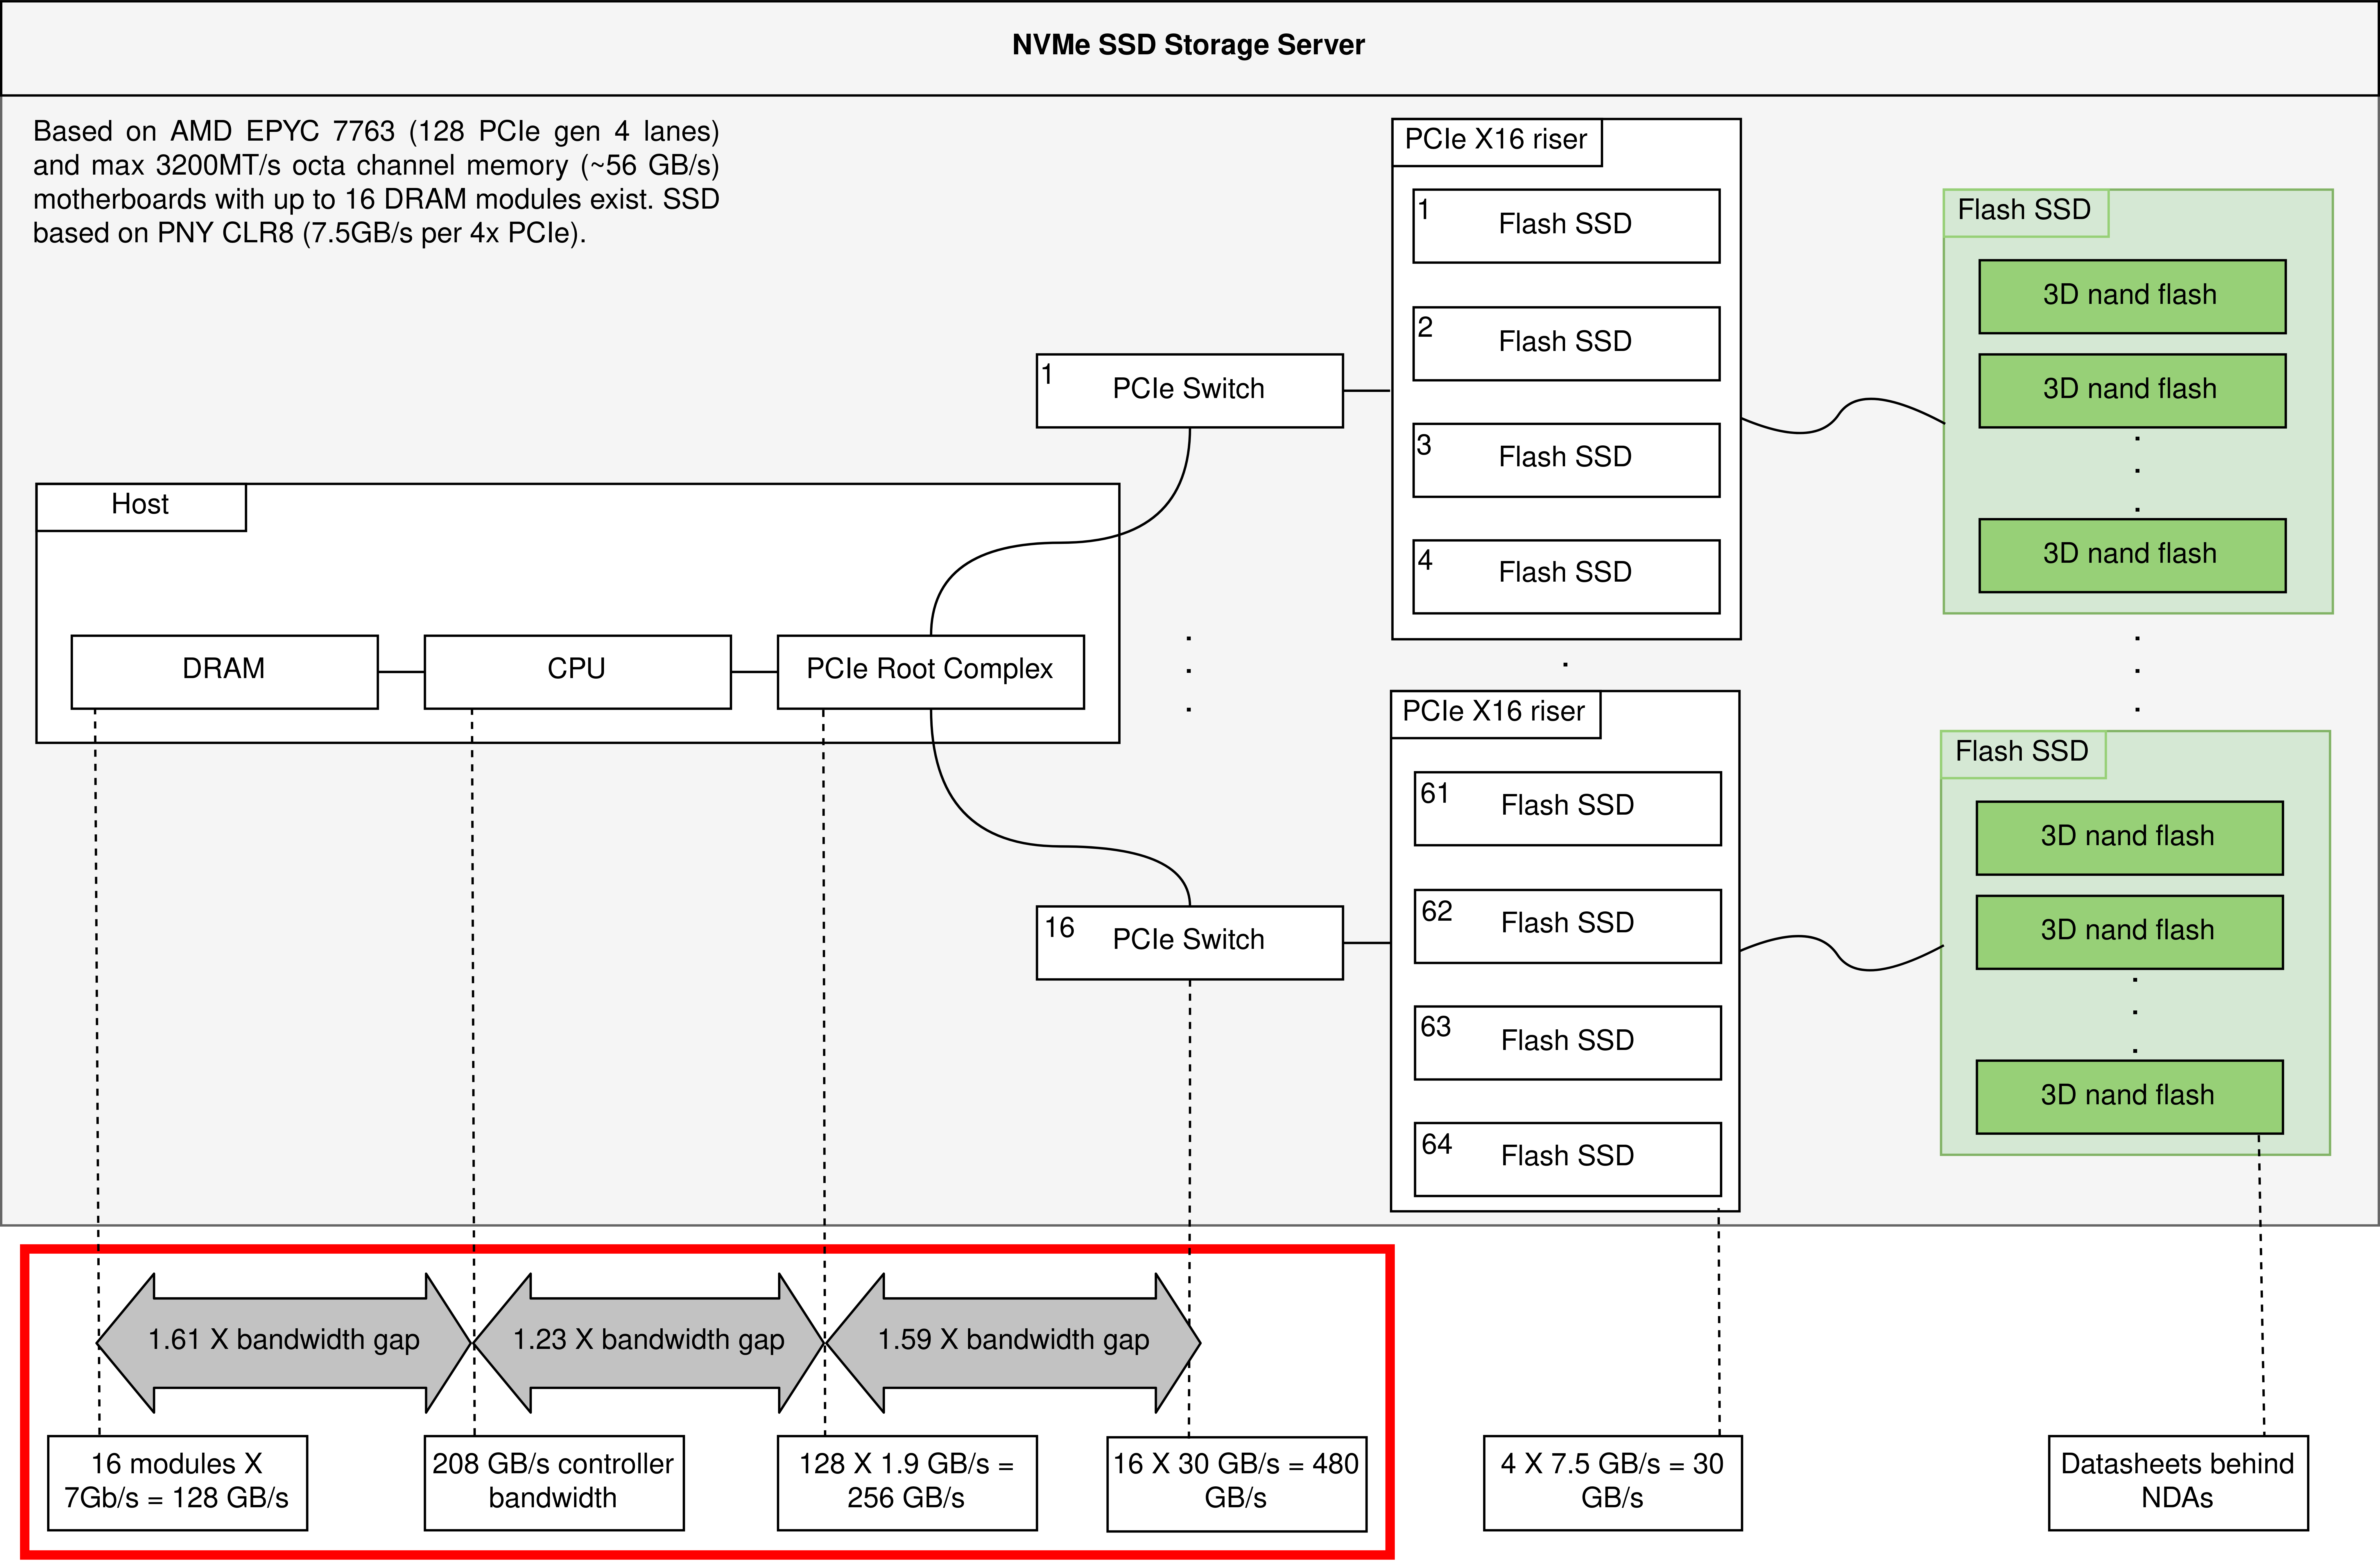
\includegraphics[width=1\textwidth]{resources/images/storage-bottleneck.png}
	\caption{Typical bandwidth limitations in modern storage servers using 64
        SSDs.}
    % \includesvg[width=0.6\columnwidth]{resources/images/module-dependencies}
    \label{figure:storagebottleneck}
\end{figure}

% Potential solution and benefits

A promising solution to this problem is the processing of data in-situ by
pushing compute to the storage layer. This solution is actively being researched
as \textit{"Programmable Storage"} and \textit{"Computational Storage"} among
other terms. The concept is not new however, as it has been previously
explored in database mainframes \cite{database-computer} as well as for
conventional HDDs \cite{active-disk-pillar, active-disks-tech,
intelligent-disk}. With the rise of Non-Volatile Memory Express (NVMe)
technologies offering significantly more device-internal bandwidth this concept
is being revisited. What makes NVMe SSDs even more suited is that they already
contain capable processing units often boasting even multiple cores. This
requirement comes from the internal management the device has to perform known
as the \textit{Flash Translation Layer} (FTL). Devices utilizing computational
elements on conventional SSDs for \textit{Computational Storage} are commonly
known as \textit{Computational Storage Devices} (CSx)s. The potential benefits
of such a heterogeneous architecture offering programmable storage include
energy saving, cost reduction and performance improvements.

% Challenges

Despite all these benefits there is still no widespread adoption even after a
decade of research \cite{lukken2021past}. A multitude of challenges
have prohibited this adoption of which several are still applicable today. Four
prominent challenges include that, firstly, \textit{Computational Storage}
requires complete vertical integration. Meaning that changes are required at all
levels of abstraction, device hardware, interfaces, drivers and operating system
to name a few. Trying to integrate a solution for all levels in one prototype
results in a very large problem space. This large problem space complicates
deriving standards for designs and interfaces although the development of such a
standard by SNIA is on-going \cite{snia-model}. Secondly, vendors might choose
to use different hardware with different
\textit{Instruction Set Architectures} (ISA)s or different host-to-device
interfaces. These differences might result in incompatible user applications
across vendors hurting reusability and hindering adoption. Third, filesystems
are managed by the host operating system while the FTL is
managed by the device. Given that one is not aware of the processes within the
other, this semantic gap complicates several aspects such as consistency,
concurrency, multi-user tenancy and filesystem integration. Lastly, no
specialized filesystem designs exist that support both regular user access
concurrent with \textit{Computational Storage} offloading.

% Solutions

In this work we address each of these challenges directly and propose a
complete \textit{Computational Storage} solution that offers a filesystem
capable of concurrent regular and computationally offloaded access (hybrid).
We introduce each of the solutions briefly before describing their complete
case. Firstly, circumvent the complexity of complete vertical integration by
creating an emulation platform on top of QEMU \cite{qemu}. Secondly, eliminate
potential incompatibilities across vendors by using \textit{Extended Berkely
Packet Filer} (eBPF) \cite{what-ebpf} as compute kernel language. Third, bridge
the semantic gap by using \textit{Zoned Namespaces} (ZNS) \cite{zns} SSDs which
moves the FTL to the host operating system (host-managed). Lastly, allow for
concurrent \textit{Hybrid Filesystem} access by developing a specialized
\textit{Log-Structured Filesystem} (LFS) \cite{Rosenblum1992TheDA} with an
in-memory snapshot consistency model \cite{Viotti2016ConsistencyIN}. We present
this complete solution as \textit{OpenCSD} an open-source Apache 2 licensed CSx
emulation framework with accompanying filesystem called \textit{FluffleFS}
\cite{qemu-csd}.

Our work aligns with the hollistic system-wide qualities of the future Dutch
computer systems research manifesto
\cite{Iosup2018MassivizingCS, Iosup2022FutureCS}. Taking into account all four
societal challenges being, Manageability, Responsibility, Sustainability and
Usability.

Clearly computational storage is a promising avenue to the data movement
bottleneck. However, there remain clear challenges that currently prevent it
from being effective. We will describe the four cases of our solution in the
design section.


% Having mentioned the four parts of our solution briefly we
% now describe their complete cases in the next sections.

\section{Research Questions}

The main scientific contribution of this work is formulated in the form of a
research question. In addition, we formulate several sub questions which aid in
showing to which extend the main research question is answered. The sub research
questions relate both to design choices as well as qualitative performance
evaluations.

Our main scientific contribution aims to answer one of the most prominent open
research questions in the field of Computational Storage. The question of
designing a filesystem that supports both regular and offloaded access, so
called \textit{hybrid filesystems}. We formulate that into the following
research question. Namely,

\begin{displayquote}
    (R1) How to create a \textit{hybrid} LFS with concurrent regular and 
    Computational Storage offloading support?
\end{displayquote}

% Ensure the research questions are such that they support the design
% requirements.

\begin{itemize}
    \item Design Requirements
    \begin{itemize}
        \item (RD1) What existing technologies are best suited for a hybrid LFS?
        \item (RD2) What techniques can be used to minimize the complexity
              required to use a hybrid LFS?
        \item (RD3) What mechanisms allow for simplified replacement of used
              existing technologies in a hybrid LFS?
        \item (RD4) How to register CSx compute kernels using existing operating 
              system APIs?
        \item (RD5) How to differentiate individual users, files and I/O
              operations in relation to their CSx compute kernel?
        \item (RD6) How to design a compute kernel API that can be reused across
              devices?
        \item (RD7) How to ensure user submitted CSx compute kernels are safe?
    \end{itemize}
    \item Experimental Evaluation
    \begin{itemize}
        \item (RE1) Can a concurrent hybrid LFS achieve undisturbed performance
              for concurrent regular and offloaded file access?
        \item (RE2) Can a concurrent hybrid LFS reduce the data movement
              between device and host?
        \item (RE3) Can a concurrent hybrid LFS reduce the host load for
              asynchronous applications?
    \end{itemize}
\end{itemize}

Our design requirements aim to result in practical solution (RD2) that can
easily be adopted should new technologies emerge (RD3) with high ease of use
(RD2) while still allowing for concurrent regular and offloaded access
(R1, RD5, RD6, RD7). In addition, our experimental evaluation aims to show that
while doing so we can achieve the typical benefits associated with such designs
(RE1, RE2, RE3).

\section{Research Method}

A well-defined research method is needed to answer the main, design requirements
and performance evaluation research questions. Given the nature of the work,
being the development and evaluation of a research software prototype, an
iterative design approach similar to that of Agile
(M1 \cite{Schwaber2001AgileSD}) is best suited. Meanwhile the evaluation method
uses a more straightforward aproach consisting of several performance
evaluations (M2 \cite{Jain1991TheAO}). Each of these evaluations provides
insights into aspects of our concurrent hybrid LFS. However, we should
be careful about concluding cause and effect from our results instead only
suggesting possible future avenues for further experiments to support our
predictions. Finally, our work follows principles of open science
(M3 \cite{Wilkinson2016TheFG}).

Given the large of possible iterative design approaches we describe ours
more elaborately in the next section.

\subsection{Design Approach}

Our design approach consists of an initial step performed only once followed by
as many iterations as necessary to complete the design. The first being
identifying the critical components. Subsequently, the iterative design approach
consists of the following three steps. First, identify existing technologies
that can be used for one or more of the critical components (RD1). Secondly,
evaluate each of the potential technologies. Third, implement the
functionality of the component using the selected technology. Any issue that
prevents the further use of a chosen technology starts the next iteration of the
design process. If no alternatives can be found workarounds or practical
limitations are introduced instead. During the iterative process weekly
discussion are held with relevant stakeholders to demonstrate progress, indicate
potential problems and find solutions.

This design approach should allow for the selection of the best available
existing technologies (RD1) given the design requirements while allowing to
change any chosen technologies (RD3) during the implementation process.

\subsection{Main Contributions}

Our work contributes in three areas being \begin{enumerate*} \item conceptual
\item experimental \item artifacts \end{enumerate*}. In total this work
provides seven distinct contributions.

\begin{itemize}
    \item (Conceptual) A design of a complete userspace emulation framework
    supporting filesystem integration for concurrent regular and offloaded
    (hybrid) access.
    \item (Conceptual) A design of a hybrid userspace filesystem reusing
    existing operating system APIs.
    \item (Experimental) Characterization of the performance of an userspace
    hybrid filesystem in microbenchmarks.
    \item (Experimental) Characterization of reduction in data movement and host
    CPU load by offloading applications.
    \item (Artifact) A prototype framework and accompanying filesystem capable
    of hybrid filesystem access \cite{qemu-csd}.
    \item (Dissemination) Presentations about progression on this research
        prototype.
        \begin{itemize}
            \item ICT.OPEN 2022: OpenCSD: Unified Architecture for eBPF-powered
                  Computational Storage Devices (CSD) with Filesystem Support
                  \cite{lukken2022ictopen}
        \end{itemize}
    \item (Dissemination) Publications on earlier versions of this prototype and
        related literature.
        \begin{itemize}
            \item Past, Present and Future of Computational Storage: A Survey \cite{lukken2021past}
            \item ZCSD: a Computational Storage Device over Zoned Namespaces (ZNS) SSDs \cite{lukken2021zcsd}
        \end{itemize}
\end{itemize}